\documentclass{article}

\usepackage{marvosym}
\usepackage{amsmath}
\usepackage{amsfonts}
\usepackage{graphicx}
\usepackage{babel}
\usepackage{algorithm}
\usepackage{algpseudocode}

\graphicspath{{images/}}

\renewcommand\refname{Vir}


\author{Gašper Terglav}
\date{22. maj 2024}
\title{Najkrajša pot z odstranljivimi ovirami --  poročilo}


\begin{document}


\maketitle


\section*{Predstavitev problema}

Problem je posplošitev klasične verzije, v kateri se lahko oviram samo izogibamo. V $\mathbb{R}^2$ imamo dve točki s in t iščemo najkrajšo evklidsko pot med njima. Ovire v ravnini so konveksni večkotniki, vsak od njih ima ceno $c_i > 0$. Če imamo na voljo $C$ ''denarja'', katere ovire se splača odstraniti, da dosežemo najkrajšo pot? V resničem življenju lahko npr.\ načrtovalci mest spremenijo cestno omrežje, da dosežejo boljšo pretočnost in tako odstranijo ovire za neko ceno. Še en primer omenjen v članku so skladišča v katerih delajo roboti. Kako spremeniti postavitev ovir v skladišču, da se roboti hitreje premikajo okoli? 

Preprost primer na katerem so ovire s cenami, začetek in konec, ter proračun lahko vidimo na sliki \ref{fig:errPr1}.

\begin{figure}[h]
    \centering
    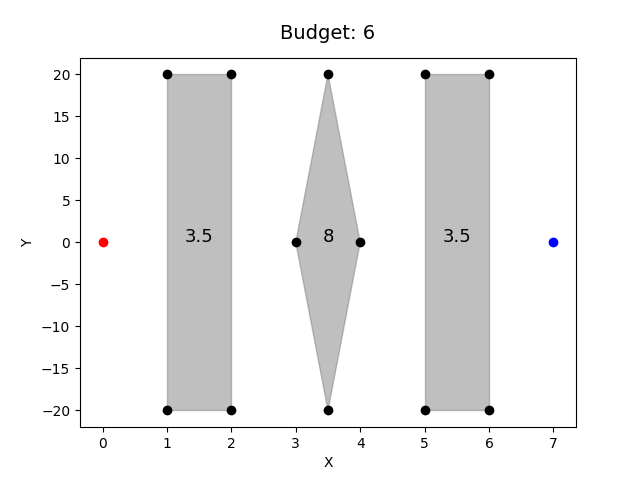
\includegraphics[width=0.65\textwidth]{err1.png}
    \caption{Primer problema.}
    \label{fig:errPr1}
\end{figure}


Zanima nas torej: ali obstaja pot dolžine $L$ in cene $C$ med začetkom in koncem? Ta problem je na žalost NP-težek, zato se bomo za polinomski čas morali zadovoljiti z algoritmom, ki ima neko napako vsaj v ceni. Še pred algoritmi iz članka pa je treba narediti t.~i.\ "viability graph" za naš problem.



% \subsection*{NP-težkost}

% Naš problem je NP-težek. To pokažemo z redukcijo na problem PARTITION, ki je NP-poln. Pri tem problemu imamo množico $A = \{a_1, a_2, ..., a_n\}$ pozitivnih celih števil. Vprašanje je, ali lakho $A$ razdelimo v množici $A_1$ in $A_2$, tako da je $W(A_1) = W(A_2) = \frac{1}{2}W(A)$, kjer je $W(S)$ vsota vseh elementov v $S$. Redukcijo dosežemo tako, da med točki $s$ in $t$ postavimo $n$ ovir, tako da je cena odstranitve enaka dolžini, za katero se pot podaljša, če ovire ne odstranimo. Če obstaja pot med s in t dolžine $\frac{1}{2}W(A) + \lVert s - t \rVert$ , kjer imamo $\frac{1}{2}W(A)$ proračuna za odstranitev ovir, potem smo našli razdelitev $A$ na dva enaka dela. Ovire, ki smo jih odstranili damo v eno možico, ostale pa v drugo.  

\section*{Algoritmi}

\subsection*{Viability graph}

Začnimo s pomembnima opazkama o obnašanju najkrajše poti. Če bo šla naša pot skozi oviro, bo zaradi konveksnosti sekala samo dve stranici večkotnika. Smer bo pot spremenila samo v ogliščih večkotnikov. Tako bomo lahko problem prevedli na iskanje najkrajše poti v grafu, katerega vozlišča so vsa oglišča ovir ter točki $s$ in $t$. Označimo ta graf z $G = (V, E)$, kjer $(u,v) \in E$, če je vsota cen vseh ovir, ki jih prečka daljica $\overline{uv}$ manjša ali enaka od našega proračuna $C$. Vsaka povezava v grafu ima dva parametra, dolžino in ceno. 

Najprej sem se konstrukcije lotil naivno. Za vsak par točk sem za vsako oviro pogledal, če jo pot seka. Ta pristop ima časovno zahtevnost $O(n^3)$. Je pa tudi veliko robnih primerov, ki otežijo implementacijo. Trenutna implementacija ima problem, ko je na poti med ogliščema še tretje oglišče. Če sta drugo in tretje oglišče del iste ovire in gre pot po njeni notranjosti, tega nisem znal na lep način zaznati. Tako bi imela ta povezava premajhno ceno. Implementacija je v datoteki "viabilityGraph.py"

Viabilty graph je v resnici posplošitev konstrukcije z imenom angleškim imenom visibility graph, s katerim se rešuje osnovno verzijo problema, kjer je $C = 0$. O tej verziji je več literature, s katero sem si lahko pomagal. Zato sem izgradnjo visibility grapha iz knjige~\cite{BCKO} v poglavju $15$ posplošil na viability graph. 
Na vsakem koraku pri konstrukciji izberemo novo oglišče $v$. Ugotoviti moramo, do katerih oglišč lahko iz $v$ pridemo s ceno največ $C$. Pri naivnem pristopu smo oglišča pregledali kakor so padla. Sedaj pa jih hočemo v nekem pametnem vrstnem redu, da bomo lahko nekaj informacij uporabili za naprej. Predstavljajmo si poltrak $p$, ki ima izhodišče v $v$ in naredi en krog v smeri urinega kazalca. Oglišča bomo pregledali v vrstnem redu, ki ga določa ta sprehod poltraka (ang.\ plane sweep). Če $p$ oglišča seka istočasno, imajo prednost tista, ki so bližje $v$.
Robove ovir, ki jih $p$ seka, bomo shranili v dvojiško drevo, kar omogoča hitrejše dodajanje in brisanje.

\begin{algorithm}
    \caption{Vrnem seznam oglišč, ki jih lahko dosežemo iz $v$}
    \begin{algorithmic}[1]
        \State Uredimo preostala oglišča glede na kot, ki ga daljica med ogliščem in $v$ naredi s pozitivno x-osjo.
        \State  Dodamo v drevo vse robove, ki jih $p$ seka. Prvi rob je tisti, ki ga poltrak najprej seka.
        \State $W$ = [ \ ]
        \For{ $w_i$ v urejenih ogliščih } 
        \If{(cena poti med $v$ in $w_i$) $\leq C$}
            \State Dodamo $w_i$ v $W$.
        \EndIf
        \State Zavrtimo poltrak $p$, da gre sedaj še skozi $w_i$.
        \State Odstranimo iz drevesa robove ovir, ki se končajo v $w_i$ ter ležijo nad $p$.
        \State Dodamo v drevo robove, ki se končajo v $w_i$ in ležijo pod njim.
        \EndFor
        \State \Return $W$
    \end{algorithmic}
\end{algorithm}

Ta algoritem poženemo za vsako oglišče, ki ga imamo in tako lahko sestavimo naš viability graph. Potrebujemo pa še funkcijo, ki nam v 5. koraku izračuna ceno poti. Kot argument ji moramo podati točke $v$, $w_i$, $w_{i-1}$ ter ceno poti $vw_{i-1}$ in še naše dvojiško drevo ter vse ovire. Ključno je, da če $w_i$ in $w_{i-1}$ ležita na isti premici, lahko uporabimo to kar vemo o $w_{i-1}$.

Ta funkcija z imenom \emph{viable} nato za vsak $w_i$ pregleda dvojiško drevo in sešteje cene vseh ovir, ki jih $vw$ seka. Že to je počasneje kot v verziji problema, ko je $C = 0$. Tam nas večino časa zanima samo rob z najmanjšim ključem v drevesu. Ta je najbližje $v$. Če obstaja in seka $\overline{vw_i}$ potem $w_i$ seveda ni viden. Celotno drevo pregledujemo tam samo, če sta $w_i$ in $w_{i-1}$ kolinearna in je $w_{i-1}$ viden. In tudi v tem primeru iščemo samo do prvega presečišča. Drugi problem je, da moramo vsakič na začetku preveriti, ali sta $v$ in $w_i$ del iste ovire. V trenutni implementaciji se tega lotim naivno, kar ima zahetvnost $O(n)$. Zaradi tega je zahtevnost celotnega algoritma skupaj spet $O(n^3)$, kljub temu da je zahtevnost tistega v \cite{BCKO} le $O(n^2 \log n)$. Prvi korak v izboljšavi algoritma je torej nov algoritem, ki preveri če sta dve oglišči del iste ovire. Implementacija se nahaja v datoteki \emph{sweepViabilityGraph.py}. Rezultat algoritma, uporabljenega na našem problemu vidimo na sliki \ref{fig:errG1}.

\begin{figure}[h]
    \centering
    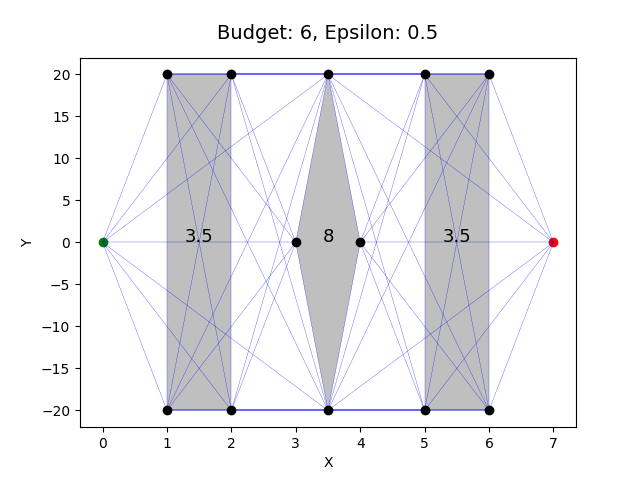
\includegraphics[width=0.65\textwidth]{errGraph1.png}
    \caption{Viability graph.}
    \label{fig:errG1}
\end{figure}

% \begin{algorithm}
%     \caption{Vrnem ceno poti med $v$ in $w_i$}
%     \begin{algorithmic}[1]
%         \If{$v$ in $w_i$ del iste ovire}
%             \If{sta soseda}
%                 \State \Return 0
%             \Else
%                 \State \Return \texttt{cena ovire}
%             \EndIf
%         \ElsIf{$v$, $w_i$, $w_{i-1}$ niso kolinearne}
%             \State  Pregledamo drevo z robovi ovir in seštejemo cene ovir, ki jih seka $\overline{vw_i}$
%             \State \Return \texttt{cena poti}
%         \Else
%             \State \texttt{cena = cena poti do $w_{i-1}$} 
%             \If{$w_i$ in $w_{i-1}$ v isti oviri}
%                 \If{$w_i$ in $w_{i-1}$ soseda v isti oviri} 
%                     \State \Return \texttt{cena}
%                 \Else
%                     \State \Return \texttt{cena + cena ovire}
%                 \EndIf
%             \Else
%             \State  Pregledamo drevo z robovi ovir in seštejemo cene ovir, ki jih seka $w_iw$
%             \State \Return \texttt{cena + cena poti $w_iw$}
%             \EndIf
%         \EndIf
%     \end{algorithmic}
% \end{algorithm}
 


\subsection*{Algoritem v polinomskem času z napako $(1+\epsilon)$ v ceni}

Ker imamo viability graph $G = (V,E)$, lahko končno začenmo z vsebino članka. Glavni problem je, da imajo povezave v $G$ dva parametra: ceno in dolžino.
Graf bi radi modificirali tako, da bi na novem grafu samo pognali Dijkstra algoritem in dobili rešitev, zato hočemo nekako odstraniti cene iz povezav. 

Naj bo  zaradi preprostosti $K = min(\frac{C}{min_i \ c_i}, h)$, kjer je $h$ število ovir, $c_i$ pa njihove cene ter $\sum c_i = C$. Delimo vse cene z $K/C$, da je naš proračun za ovire na tako enak $K$. Potem naredimo $ \lceil{\frac{2K}{\epsilon}}\rceil + 1$  kopij vsakega vozličša v grafu $G$ in jih označimo z $v_0, v_{\epsilon/2}, v_{\epsilon}..., v_K$. Za vsak rob $(u, v) \in E$ s ceno $c$ in za vsak $0 \le i \le \lceil{\frac{2K}{\epsilon}}\rceil $, dodamo rob $(u_{i \epsilon/2}, v_{j \epsilon/2})$, kjer je $j\le\lceil{\frac{2K}{\epsilon}}\rceil$ največje celo število da velja $j\frac{\epsilon}{2}
 \le i \frac{\epsilon}{2} + c$. Dolžina povezav je enaka kot v originalnem grafu. Tako smo ceno zakodirali v vozlišča. Indeks v vozlišču nam pove, koliko smo plačali na poti do sedaj. Na koncu dodamo še novi vozlišči $s$ in $t$, ter vsakega od njiju povežemo z vsemi njunimi kopijami. Te povezave imajo dolžino $0$. Ker imajo povezave samo še dolžino, lahko sedaj za iskanje najkrajše poti uporabimo Dijkstro. Novi graf ima $O(|V|K/\epsilon)$ vozlišč in $O(|E|K/\epsilon)$ robov. Dijkstra  je  časovno najbolj zahtevna stvar, zato je časovna zahtevnost celotnega algoritma enaka $O(\frac{K}{\epsilon}(|E| + |V|\log\frac{|V|}{\epsilon}) )$. Če je $n$ število vseh oglišč ovir, je to v najboljšem primeru $\Omega(\frac{n^3}{\epsilon})$.

 Tako lahko končno najdemo najkrajšo pot pri našem problemu, prikazano na sliki \ref{fig:errP1}.

 \begin{figure}[h]
    \centering
    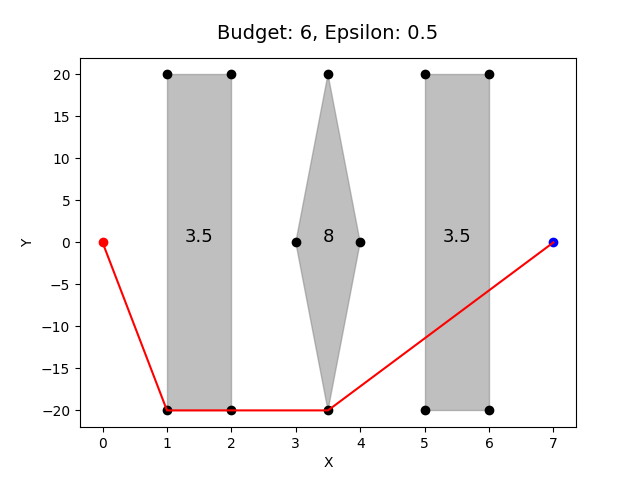
\includegraphics[width=0.65\textwidth]{errPath1.png}
    \caption{Najkrajša pot z $\epsilon = 0.5$.}
    \label{fig:errP1}
\end{figure}

V svoji implementaciji zaradi preprostosti ne naredim $2/\epsilon$ kopij temveč samo $1/\epsilon$. Posledično bo cena najkrajše poti manjša od $(1 + 2\epsilon)C$. Čeprav je naš primer zelo preprost, se napaka pojavi če izberemo $\epsilon > 0.5$, kot vidimo na sliki \ref{fig:errP05}.

\begin{figure}[ht]
    \centering
    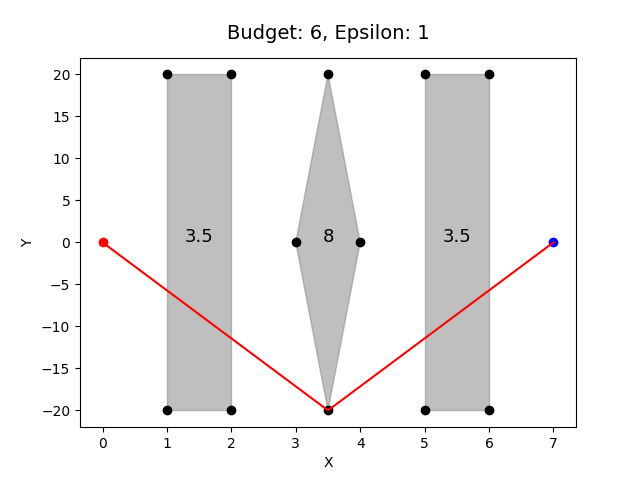
\includegraphics[width=0.65\textwidth]{errPathEps1.png}
    \caption{Najkrajša pot z $\epsilon = 1$.}
    \label{fig:errP05}
\end{figure}




\subsection*{Hitrejši algoritem}

Za večjo hitrost bomo morali modificirati graf $G$. Pravzaprav hočemo zmanjšati število povezav v grafu, na katerem na koncu poženemo Dijsktro. V zameno pa je tukaj lahko napaka $(1+\epsilon)$ tudi pri dolžini poti. Algoritem ima dva dela. Najprej konstruiramo nov graf $H = (X,\Gamma)$, ki bo imel manj povezav kot $G$. Zanimivo pa je, da ima $H$ več vozlišč kot $G$. K drugem delu pristopimo podobno kot prej, s kopiranjem grafa $H$. Ta algoritem ima časovno zahtevnost $O(\frac{nh}{\epsilon^2}\log n \log \frac{n}{\epsilon})$ kar je približno za potenco $n$ manj kot prejšnji algoritem.

\subsubsection*{Konstrukcija grafa $H$}

Začeli smo z grafom $G = (V,E)$. Za $H = (X,\Gamma)$ bo veljalo $|X|, |\Gamma| = O(n \log n)$ in $V \subseteq X$. Označimo razdaljo med ogliščema $v,u$ v grafu $G$ z $d_G(v,u)$. Potem bo za vsak par $v,u \in G$ veljalo  $d_G(v,u) \leq d_H(v,u) \leq \sqrt{2}d_G(v,u)$. Naše poti bodo sestavljene bolj iz vodoravnih in navpičnih segmentov, jih bo pa manj.

Graf $H$ konstruiramo z naslednjim rekurzivnim algoritmom.

\begin{algorithm}
    \caption{Dobimo graf $H$ z manj povezavami}
    \begin{algorithmic}[1]
        \State Naj bo $x_m$ mediana za $x$-koordinate točk v $V$. 
        \State  Naj bo $l_v: \ x = x_m$ navpična premica, ki razdeli $V$ na levo polovico $V_l$ in desno $V_d$.
        \For{ $v \in V$} 
            \State Dobimo projekcijo $v' = (x_m,v_y)$
            \If {cena poti $\overline{vv'} \leq C$}
                \State Dodamo $v'$ v $X$ in $(v,v')$ v $\Gamma$
            \EndIf
            \State Naj bo $s'$ prvi rob ovire s pozitivnim naklonom, ki seka $\overline{vv'}$. 
            \If{$s'$ seka $l_v$} 
                \State Dodali bomo "obhodna" vozlišča in povezave v $H$.
                \State Označimo presečišče $\overline{vv'}$ in $s'$ z $v_1$ in presečišče $s'$ in $l_v$ z $v_2$. 
                \State Dodamo ti dve točki v $X$ ter povezavi $(v,v_1)$ in $(v_1,v_2)$ v $\Gamma$.
            \EndIf
            \State Ponovimo postopek za prvi $s'$ z negativnim naklonom.
            \State Recimo točkam na premici $l_v$ Steinerjeve točke.
            \For{$w, w'$ sosednji Steinerjevi točki}
                \State Če je cena $\overline{ww'} \leq C$, dodamo $(w,w')$ v $\Gamma$.
            \EndFor
        \EndFor
        \State Rekurzivno ponovimo na množicah $V_l$ in $V_d$.
        
        \State Ponovimo vse zgoraj, le tokrat z mediano $y_m$ za $y$-koordinate  in premico $l_h: \ y_m = y$.
        \State Dodamo v $\Gamma$ še robove ovir.
    \end{algorithmic}
\end{algorithm}


\begin{thebibliography}{99}

    \bibitem{PNS} P.~K.~Agarwal, N.~Kumar, S.~Sintos in S.~Suri. \emph{Computing Shortest Paths in the Plane with Removable Obstacles}. In 16th Scandinavian Symposium and Workshops on Algorithm Theory (SWAT 2018). Leibniz International Proceedings in Informatics (LIPIcs), Volume 101, pp. 5:1-5:15, Schloss Dagstuhl – Leibniz-Zentrum für Informatik (2018)

    \bibitem{BCKO} M.~Berg, O.~Cheong, M.~Kreveld in  M.~Overmars \emph{Computational Geometry: Algorithms and Applications} Springer Berlin, Heidelberg, 2010

\end{thebibliography}
\end{document}